\documentclass[12pt,a4paper]{ctexart}
\usepackage[a4paper,top=2.2cm,bottom=2.2cm,left=2.2cm,right=2.2cm,headheight=15pt]{geometry}
\usepackage{graphicx}
\usepackage{booktabs}
\usepackage{array}
\usepackage{xcolor}
\usepackage{enumitem}
\usepackage{listings}
\usepackage{fancyhdr}
\usepackage{caption}
\usepackage{float}
\usepackage{hyperref}

\hypersetup{colorlinks=true,linkcolor=black,urlcolor=blue,citecolor=black}

\lstset{
  basicstyle=\ttfamily\small,
  breaklines=true,
  frame=single,
  columns=fullflexible,
  keepspaces=true,
  showstringspaces=false,
  keywordstyle=\color{blue},
  commentstyle=\color{green!50!black},
  stringstyle=\color{red!60!black},
  numberstyle=\tiny\color{gray},
  numbers=none,
  aboveskip=6pt,
  belowskip=6pt
}

\captionsetup{font=small,labelfont=bf,justification=centering}

\pagestyle{fancy}
\fancyhf{}
\fancyhead[L]{中国海洋大学 $|$ 机器人集成小组项目1 $|$ Lab1}
\fancyhead[R]{第 \thepage 页}
\fancyfoot[C]{黄博宇 24020036026 $|$ Lab1 实验报告}
\renewcommand{\headrulewidth}{0.4pt}
\renewcommand{\footrulewidth}{0.4pt}

\setlength{\parindent}{2em}
\setlength{\parskip}{2pt}
\setlength{\emergencystretch}{3em}

\title{}
\author{}
\date{}

\begin{document}

% ==================== 封面 ====================
\begin{titlepage}
\thispagestyle{empty}
\vspace*{1.2cm}
\begin{center}
  {\Large 中国海洋大学}\\[6pt]
  {\large 机器人集成小组项目1 · Lab1 实验报告}\\[26pt]
  {\LARGE\bfseries Linux、C++ 与 Git 开发环境配置及\\[4pt] RandomVector 实现实验}\\[30pt]
\end{center}

\begin{center}
\renewcommand{\arraystretch}{1.6}
\begin{tabular}{>{\bfseries}l l}
姓名 & 黄博宇 \\
学号 & 24020036026 \\
班级 & 24级中外计科一班 \\
课程 & 机器人集成小组项目1 \\
实验名称 & Lab1 Linux、C++、Git 与 RandomVector \\
实验时间 & 2026 年 9 月 27 日 \\
实验平台 & MacBook Air + VMware Fusion \\
操作系统 & Ubuntu 20.04.5 LTS / ARM64 \\
个人仓库 & \url{https://github.com/hbyhby123/vnav-personal} \\
课程仓库 & \url{https://github.com/ouc-vlab-course/vnav-codes} \\
\end{tabular}
\end{center}

\vspace{14pt}
\begin{center}
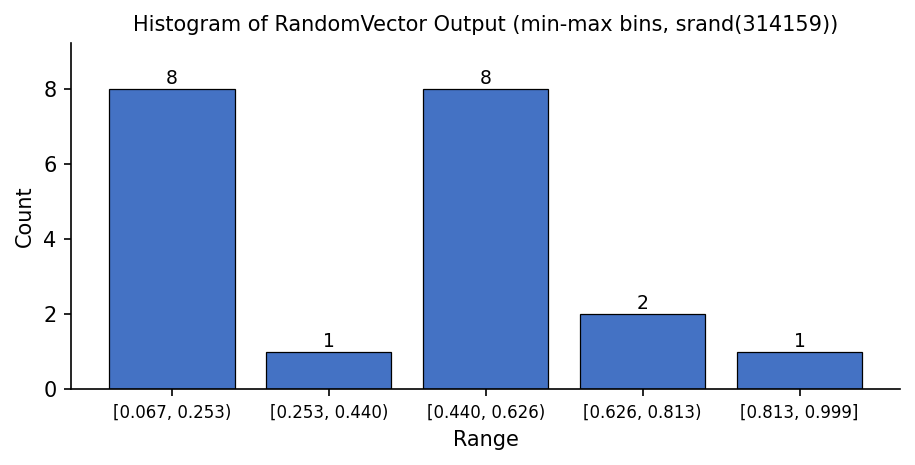
\includegraphics[width=0.66\textwidth]{figures/fig_hist_new.png}\\[4pt]
{\small\bfseries 图 0 \quad Lab1 最终运行结果直方图（min--max 等宽分箱，固定随机种子）}
\end{center}

\vspace{10pt}
\begin{center}
\fbox{\parbox{0.86\textwidth}{\small
\textbf{实验主线：}完成 Ubuntu 20.04 安装与清华软件源配置 $\rightarrow$ Linux 基础命令 $\rightarrow$ Git 版本管理
$\rightarrow$ C++ 编译与 CMake 多文件构建 $\rightarrow$ 课程仓库与个人提交仓库 $\rightarrow$ Shell 练习
（dante.txt 统计、fortune 追加） $\rightarrow$ C++ 热身题 $\rightarrow$ RandomVector 功能实现与验证。}}
\end{center}
\end{titlepage}

% ==================== 摘要与目录 ====================
\section*{摘要与报告结构}
\addcontentsline{toc}{section}{摘要与报告结构}

\noindent\textbf{摘要：}本实验围绕机器人软件开发的基础工具链展开，依次完成 Ubuntu 20.04.5 ARM64 虚拟机创建与登录、软件源备份与清华源切换、必备工具安装（build-essential / CMake / Git）、Linux 基本命令练习、Git 版本管理入门、C++ 单文件编译、CMake 多文件工程构建，以及课程仓库（ouc-vlab-course/vnav-codes）与个人提交仓库（hbyhby123/vnav-personal）的克隆与推送。练习部分完成 Shell 练习 1（dante.txt 行/词/非空行统计）、Shell 练习 2（fortune 输出追加）、C++ 热身题作答。核心编程任务是补全 RandomVector 类的 6 个成员函数：生成随机数、输出序列、计算平均值、寻找最大值与最小值，并以 min() 与 max() 之间的等宽区间打印竖向直方图。最终程序在固定随机种子 std::srand(314159) 下稳定输出 20 个随机数及统计结果，与课程示例一致，完成了从环境搭建到代码验证的完整流程。

\vspace{4pt}
\noindent\textbf{关键词：}Ubuntu 20.04 · 清华软件源 · Linux · Git · C++ · CMake · MIT VNAV-Labs · RandomVector

\vspace{6pt}
\tableofcontents

\vspace{8pt}
\noindent\textbf{实验完成情况}
\begin{center}
\begin{tabular}{ll}
\toprule
模块 & 完成情况 \\
\midrule
Ubuntu 20.04.5 ARM64 虚拟机安装与登录 & 完成 \\
软件源备份与清华源切换 & 完成 \\
build-essential / CMake / Git 安装与验证 & 完成 \\
Linux 基础命令 & 完成 \\
Git init / add / commit / log / clone / push & 完成 \\
g++ 单文件编译 & 完成 \\
CMake 多文件工程构建（lab1\_demo） & 完成 \\
课程仓库 vnav-codes 与个人仓库 vnav-personal & 完成 \\
Shell 练习 1：dante.txt 统计 & 完成 \\
Shell 练习 2：fortune 输出追加 & 完成 \\
C++ 热身题（Operators / References / Numbers） & 完成 \\
RandomVector 6 个函数实现 & 完成 \\
最终运行与统计验证 & 完成 \\
\bottomrule
\end{tabular}
\end{center}

\newpage

% ==================== 1 实验目标 ====================
\section{实验目标与总体流程}

本次 Lab1 的重点不是单独完成某一条命令，而是建立机器人项目开发所需的基础工作流：能够在 Linux 中操作文件，在 Git 中管理代码，用 g++ 或 CMake 完成编译，并在课程仓库中阅读、修改和验证 C++ 程序。

\subsection{实验目标}
\begin{enumerate}[itemsep=1pt]
\item 掌握在 VMware Fusion 中创建 Ubuntu 20.04.5 ARM64 虚拟机的基本过程，并完成软件源备份与清华源切换；
\item 学会使用 ls、cd、pwd、mkdir、touch、echo、cat、wc、grep 等 Linux 基础命令；
\item 学会使用 Git 完成 clone、init、config、add、commit、log、push 等常见操作；
\item 理解 g++ 与 CMake 的作用，完成``源代码--编译--运行--验证''的基本流程，并构建多文件 CMake 工程；
\item 完成 Shell 练习：dante.txt 行数/单词数/非空行数统计，fortune 输出重定向与追加；
\item 完成 C++ 热身题：运算符、引用与指针、数值类型相关题目；
\item 根据 random\_vector.h 与 main.cpp 的接口要求，补全 random\_vector.cpp 中的 TODO；
\item 为后续机器人课程中的工程构建、代码阅读与团队协作打下基础。
\end{enumerate}

\subsection{总体流程}
\begin{center}
\small
\begin{tabular}{cccc}
\toprule
1. Ubuntu 环境 & 2. 清华换源 & 3. 工具安装 & 4. Linux 命令 \\
5. Git 管理 & 6. C++/CMake & 7. RandomVector & \\
\bottomrule
\end{tabular}
\end{center}

\subsection{最终验收标准}
\begin{center}
\begin{tabular}{ll}
\toprule
检查点 & 验收结果 \\
\midrule
开发工具版本可查询 & 通过 \\
软件源更新成功（清华 ubuntu-ports） & 通过 \\
Hello C++ 正常输出 & 通过 \\
Hello CMake（多文件）正常输出 & 通过 \\
课程仓库与个人仓库克隆/推送成功 & 通过 \\
dante.txt 统计与 fortune 追加完成并推送 & 通过 \\
C++ 热身题全部作答 & 通过 \\
RandomVector 编译无警告、无功能性错误 & 通过 \\
Mean / Min / Max / Histogram 正确输出且可复现 & 通过 \\
\bottomrule
\end{tabular}
\end{center}

\textbf{一句话概括：}我完成了机器人开发基础环境搭建，基于课程仓库完成 Shell 练习、C++ 热身题与 RandomVector 类实现，全部成果已推送到个人仓库。

\newpage

% ==================== 2 实验环境 ====================
\section{实验环境与工具链}

实验在 Apple 芯片 MacBook Air 上通过 VMware Fusion 运行 Ubuntu 20.04.5 LTS。系统架构为 aarch64 / ARM64，因此 Ubuntu 安装镜像与软件源均采用 ARM64 对应版本。后续所有 Linux、Git、C++ 与 CMake 操作均在该虚拟机中完成。

\begin{center}
\begin{tabular}{ll}
\toprule
项目 & 配置 / 版本 \\
\midrule
宿主机 & MacBook Air（Apple 芯片） \\
虚拟机软件 & VMware Fusion \\
客户机操作系统 & Ubuntu 20.04.5 LTS \\
系统架构 & aarch64 / ARM64 \\
C 编译器 & gcc 9.4.0 \\
C++ 编译器 & g++ 9.4.0 \\
构建工具 & CMake 3.16.3 \\
版本管理工具 & Git 2.25.1 \\
课程仓库 & ouc-vlab-course / vnav-codes \\
实验代码来源 & MIT-SPARK / VNAV-labs \\
\bottomrule
\end{tabular}
\end{center}

\begin{figure}[H]
\centering
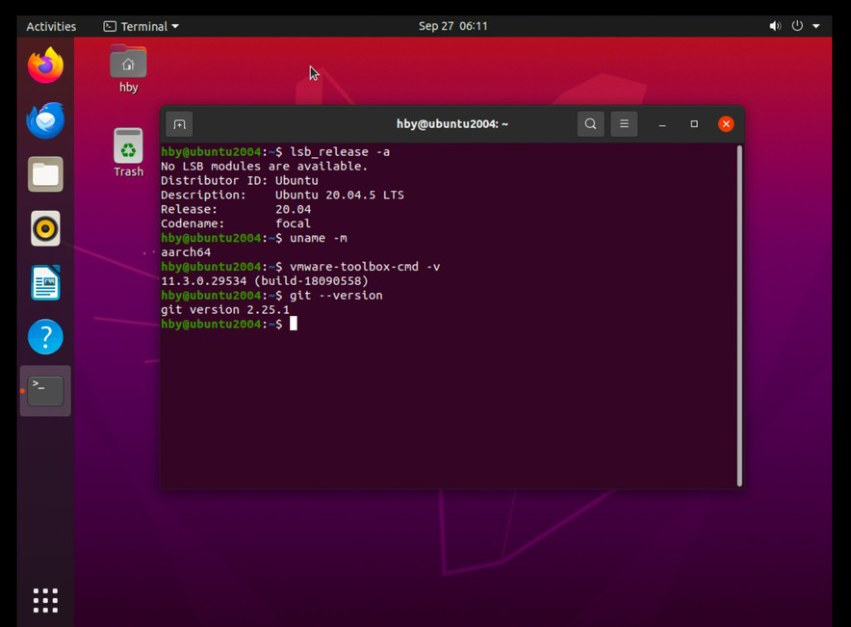
\includegraphics[width=0.42\textwidth]{figures/fig1_ubuntu.jpg}\hfill
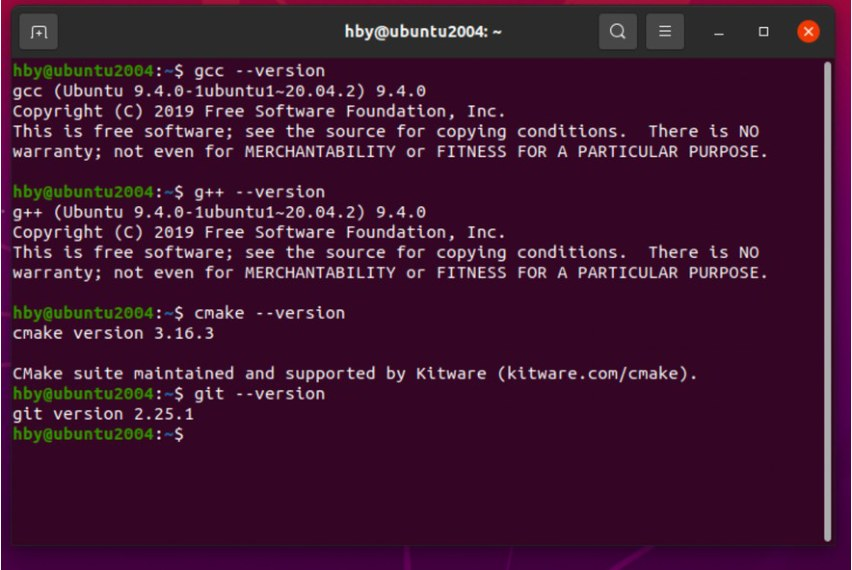
\includegraphics[width=0.44\textwidth]{figures/fig2_toolchain.jpg}
\caption{Ubuntu 版本、系统架构与工具链版本检查（lsb\_release / uname / gcc / g++ / cmake / git）}
\label{fig:toolchain}
\end{figure}

\textbf{环境验证结果：}操作系统、架构、编译器、构建工具与 Git 均可正常查询版本，说明基础工具链已经就绪。

\newpage

% ==================== 3 Ubuntu 虚拟机 ====================
\section{Part One：Ubuntu 虚拟机环境准备}

首先在 VMware Fusion 中选择 Ubuntu 20.04.5 ARM64 镜像创建虚拟机。创建完成后，系统最初以命令行方式启动，需要输入安装时设置的用户名和密码登录。完成必要配置并重启后，系统可以正常进入 Ubuntu 图形桌面。使用 lsb\_release -d 与 uname -m 核对，分别得到 Ubuntu 20.04.5 LTS 和 aarch64。

\begin{figure}[H]
\centering
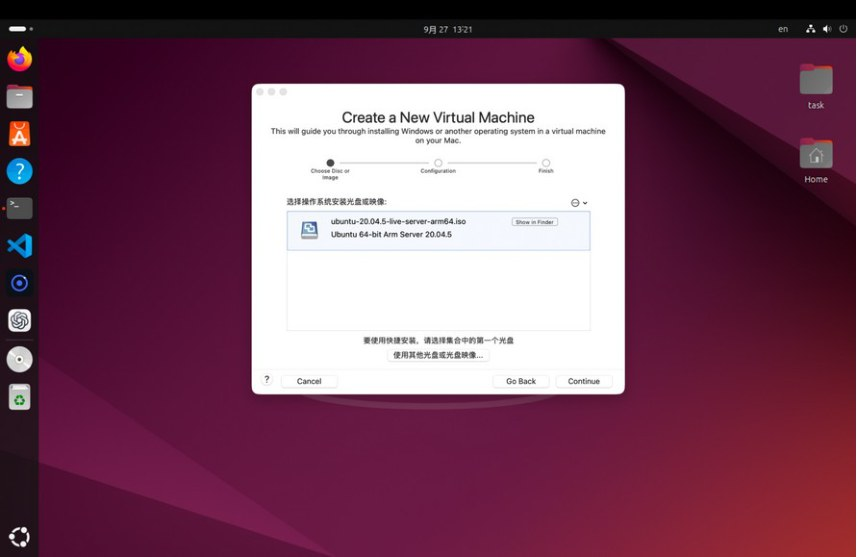
\includegraphics[width=0.40\textwidth]{figures/fig3_vmware.jpg}\hfill
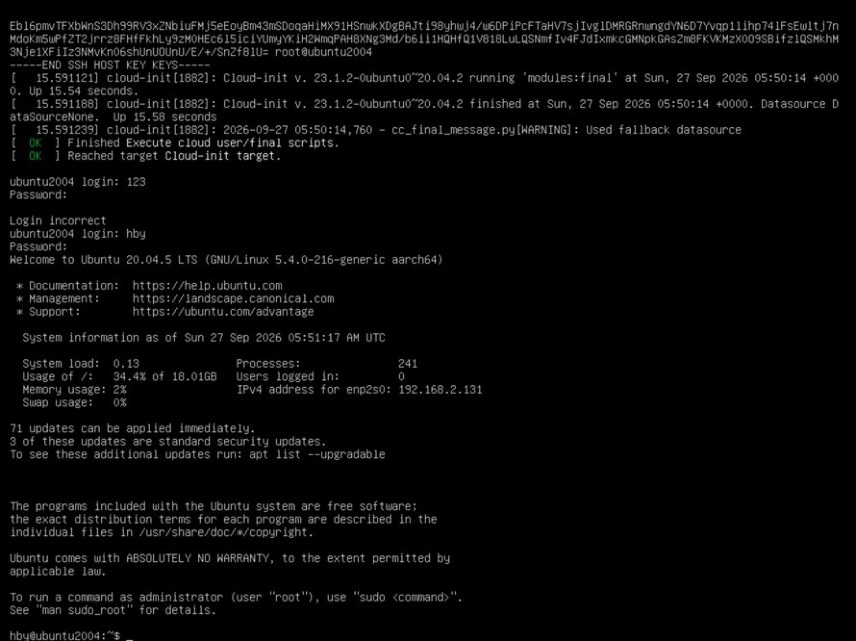
\includegraphics[width=0.40\textwidth]{figures/fig4_login.jpg}
\caption{在 VMware Fusion 中选择 Ubuntu 20.04.5 ARM64 安装镜像；首次进入命令行登录界面}
\label{fig:vm}
\end{figure}

\begin{figure}[H]
\centering
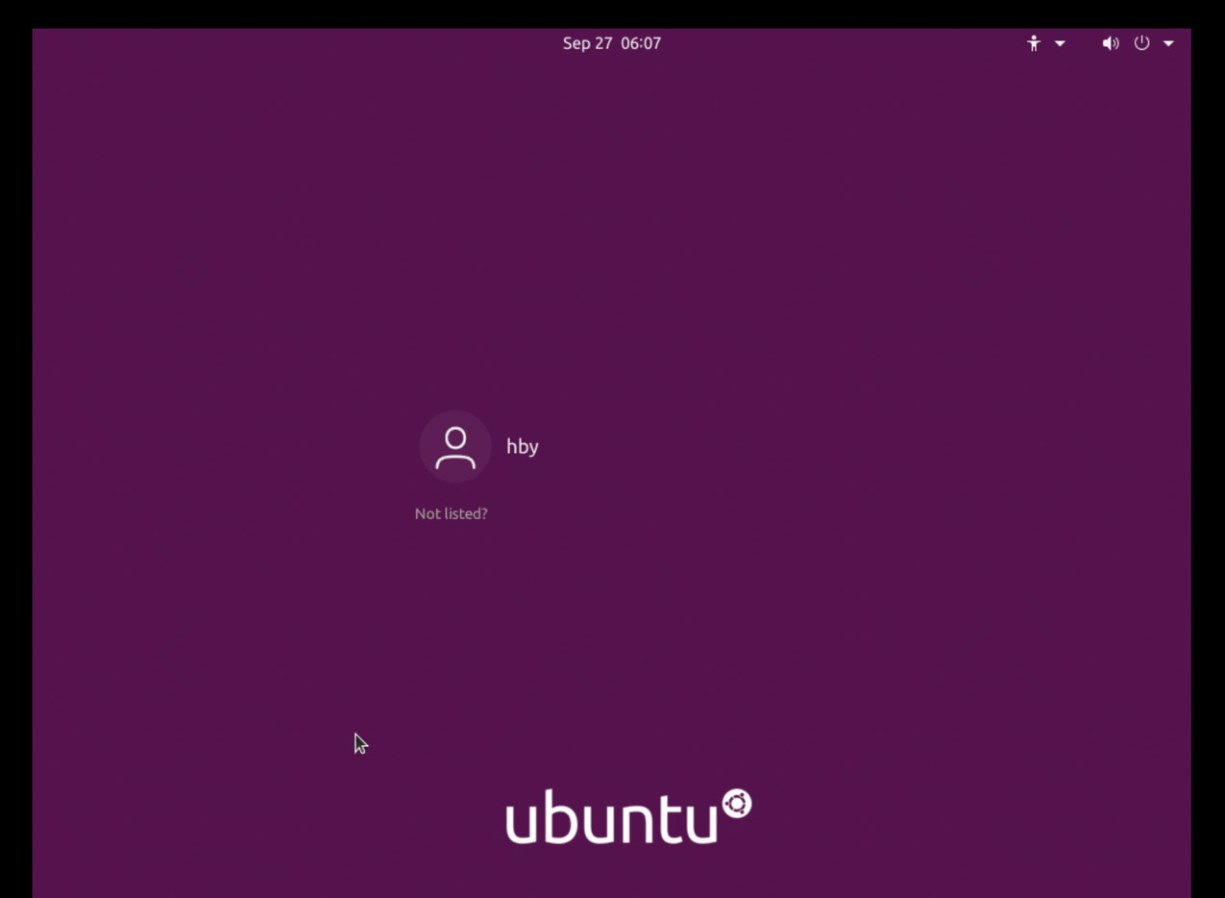
\includegraphics[width=0.52\textwidth]{figures/fig5_desktop.jpg}
\caption{重启后成功进入 Ubuntu 图形登录界面}
\label{fig:desktop}
\end{figure}

\textbf{结果分析：}虚拟机能够正常启动、登录并进入图形界面，说明 Ubuntu 环境安装完成。这个过程也说明 Linux 既可以在纯终端环境中工作，也可以在图形界面下工作。课程建议使用 NAT 网络并开启主机连接和 DHCP；本次环境能够正常访问 GitHub 和软件仓库，说明联网功能可用。

\newpage

% ==================== 4 软件源切换 ====================
\section{Part One：软件源备份与切换（清华源）}

检查发现 Ubuntu 有效源原先位于 /etc/apt/sources.list.d/original.list，使用官方 ubuntu-ports 地址。为保证下载速度与稳定性，先备份 sources.list 和 original.list，再将源地址替换为清华镜像并写入 sources.list，同时停用旧配置，避免重复启用。

\begin{lstlisting}[language=bash]
sudo cp -n /etc/apt/sources.list /etc/apt/sources.list.bak
sudo cp -n /etc/apt/sources.list.d/original.list \
  /etc/apt/sources.list.d/original.list.bak
sudo sed 's|http://ports.ubuntu.com/ubuntu-ports/|https://mirrors.tuna.tsinghua.edu.cn/ubuntu-ports/|g' \
  /etc/apt/sources.list.d/original.list | sudo tee /etc/apt/sources.list
sudo mv /etc/apt/sources.list.d/original.list \
  /etc/apt/sources.list.d/original.list.disabled
sudo apt update
\end{lstlisting}

修改后使用清华 ubuntu-ports，发行版仍为 focal，包含 focal-updates、focal-backports、focal-security 和原有组件。第三方 GitHub CLI、VS Code 配置未在本次修改中更改。

实际更新输出摘录：
\begin{lstlisting}[language=bash]
Get:1 https://mirrors.tuna.tsinghua.edu.cn/ubuntu-ports focal InRelease
Get:2 https://mirrors.tuna.tsinghua.edu.cn/ubuntu-ports focal-updates InRelease
Get:3 https://mirrors.tuna.tsinghua.edu.cn/ubuntu-ports focal-backports InRelease
Get:4 https://mirrors.tuna.tsinghua.edu.cn/ubuntu-ports focal-security InRelease
Fetched 45.2 MB in 12s (3,826 kB/s)
Reading package lists... Done
Building dependency tree
Reading state information... Done
60 packages can be upgraded.
\end{lstlisting}

\textbf{结果：}软件包索引更新成功。``60 packages can be upgraded'' 是状态提示，不代表换源失败；本步骤没有执行系统升级。sources.list.bak 备份的是原 sources.list，实际旧 Ubuntu 源另存为 original.list.bak。

\newpage

% ==================== 5 工具安装 ====================
\section{Part Two：必备工具安装与验证}

\begin{lstlisting}[language=bash]
sudo apt install build-essential cmake git
\end{lstlisting}

通过 dpkg-query 核实以下软件包均为 install ok installed：
\begin{center}
\begin{tabular}{ll}
\toprule
软件包 & 版本 \\
\midrule
build-essential & 12.8ubuntu1.1 \\
cmake & 3.16.3-1ubuntu1.20.04.1 \\
git & 1:2.25.1-1ubuntu3.14 \\
\bottomrule
\end{tabular}
\end{center}

build-essential 提供基本编译工具链；CMake 生成工程构建文件；Git 用于版本管理。第 2 章图~\ref{fig:toolchain} 中的版本截图显示 gcc/g++ 9.4.0、CMake 3.16.3、Git 2.25.1。

\textbf{验证结果：}工具安装状态正常；本次 RandomVector 的 g++ 编译和 lab1\_demo 的 CMake 构建进一步验证了工具链可用。

\newpage

% ==================== 6 Linux 命令 ====================
\section{Part Two：Linux 基础命令练习}

在 \textasciitilde/lab1 目录下，通过创建文件夹、进入目录、创建文件、写入内容和读取内容，练习 Linux 最基本的文件系统操作。重点是理解``目录--文件--路径''的关系，而不是机械记忆命令。

\begin{center}
\begin{tabular}{lll}
\toprule
命令 & 作用 & 本次实验中的用途 \\
\midrule
ls & 列出目录内容 & 检查文件/文件夹是否创建成功 \\
cd & 切换目录 & 进入 lab1、test\_folder 等目录 \\
pwd & 显示当前路径 & 确认当前位置 \\
mkdir & 创建目录 & 建立实验工作目录 \\
touch & 创建空文件 & 创建 hello.txt \\
echo & 输出/写入文本 & 向 hello.txt 写入 Hello Linux \\
cat & 显示文件内容 & 检查写入结果 \\
\bottomrule
\end{tabular}
\end{center}

\begin{figure}[H]
\centering
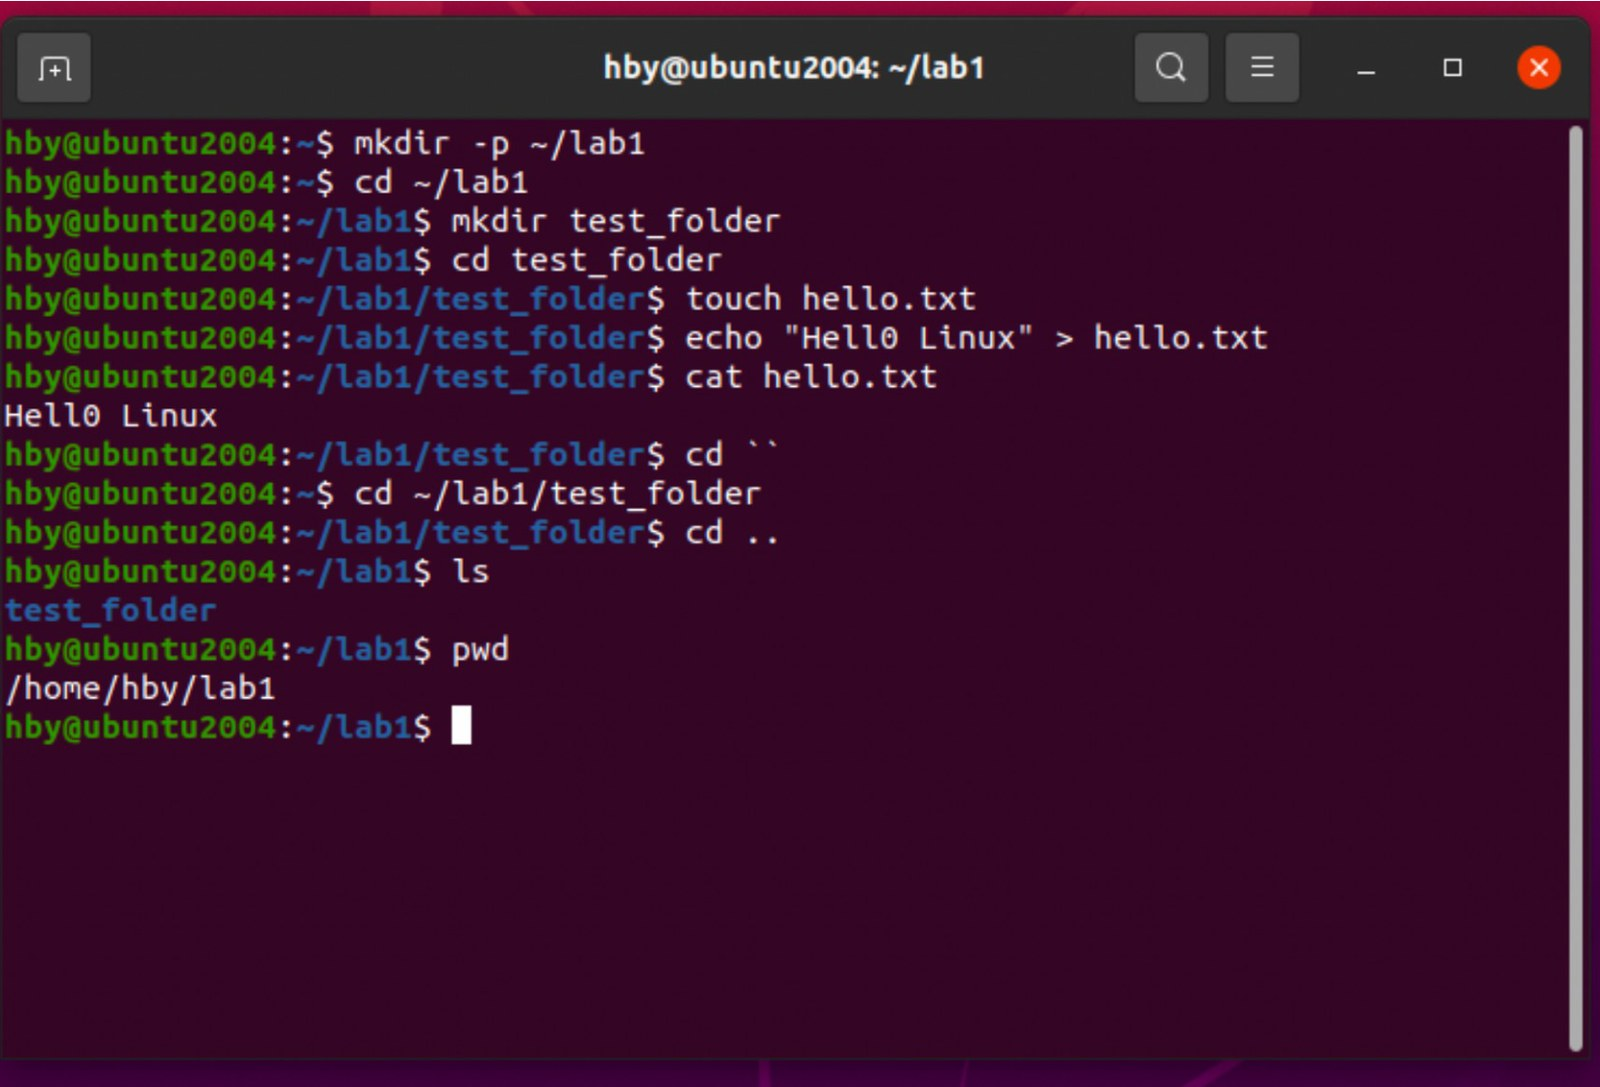
\includegraphics[width=0.62\textwidth]{figures/fig6_linux_cmds.jpg}
\caption{Linux 基本文件与目录操作练习}
\label{fig:linuxcmds}
\end{figure}

\textbf{结果：}成功创建 test\_folder 和 hello.txt，并通过 cat、ls、pwd 验证文件内容与当前路径，Linux 基础文件操作正常。

\newpage

% ==================== 7 Git 基础 ====================
\section{Part Three：Git 版本管理基础}

在 lab1\_ws 工作目录中，先执行 git init 初始化本地仓库，然后创建 README.md 测试文件。首次提交时 Git 提示缺少 user.name 与 user.email，因此按提示完成全局配置，之后成功提交，并通过 git log --oneline 查看提交历史。

\begin{lstlisting}[language=bash]
git init
git config --global user.name "hby"
git config --global user.email "..."   # 按提示填写邮箱
git add README.md
git commit -m "first commit"
git log --oneline
\end{lstlisting}

\begin{figure}[H]
\centering
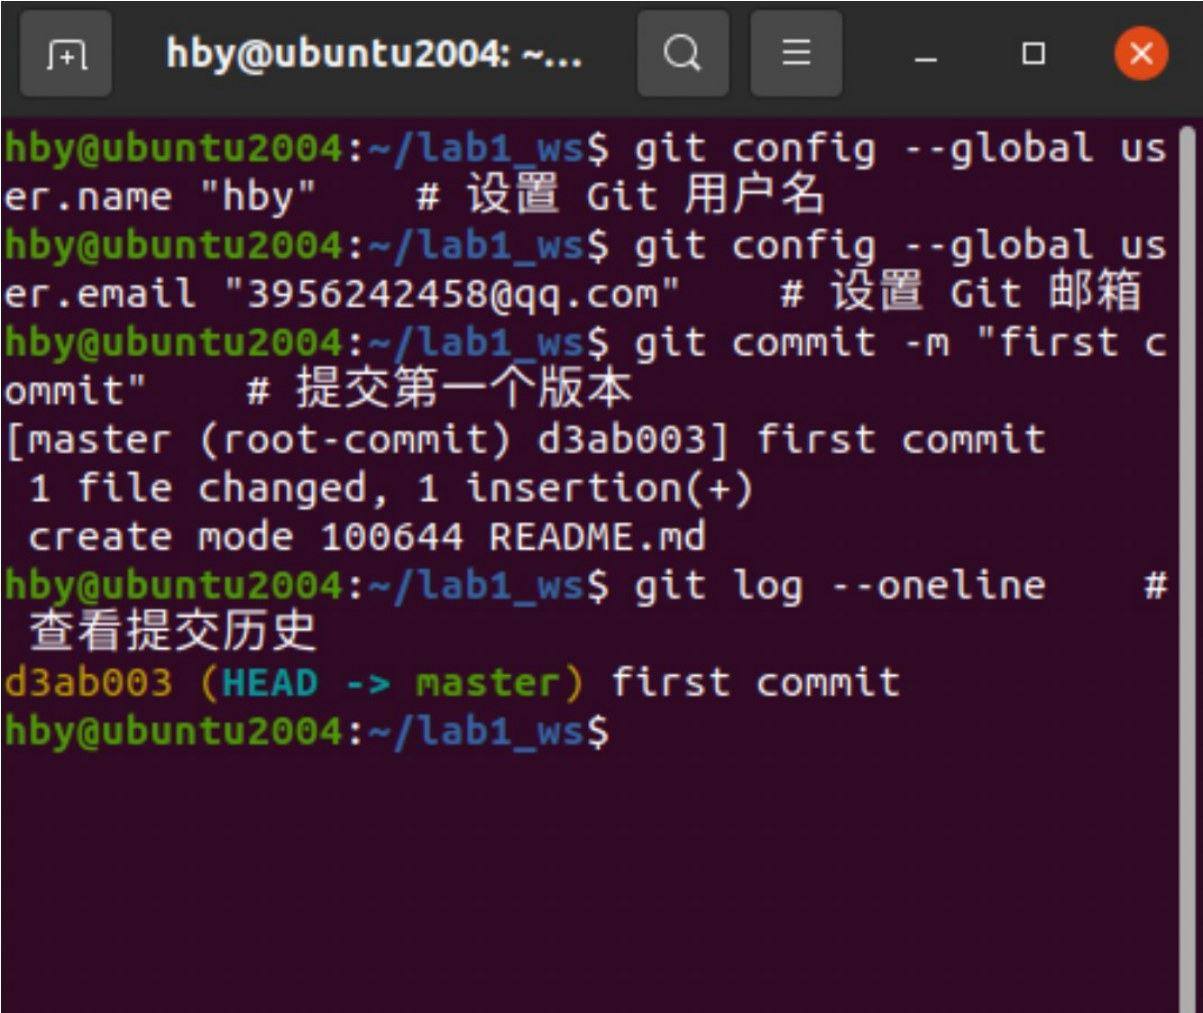
\includegraphics[width=0.52\textwidth]{figures/fig7_git.jpg}
\caption{Git 用户信息配置、首次提交与提交历史查看}
\label{fig:git}
\end{figure}

\begin{center}
\begin{tabular}{ll}
\toprule
概念 & 通俗理解 \\
\midrule
Repository & 代码仓库，用来保存项目及版本历史 \\
Commit & 一次版本快照，记录当前代码状态 \\
git add & 把准备提交的修改加入暂存区 \\
git log & 查看已经提交过的版本记录 \\
git push & 把本地提交同步到远程仓库 \\
\bottomrule
\end{tabular}
\end{center}

\textbf{本步结论：}Git 不只是``下载代码''的工具，更重要的作用是记录代码修改历史，便于个人回退和团队协作。完整流程为：clone/init 获取仓库 $\rightarrow$ status/diff 检查改动 $\rightarrow$ add 暂存 $\rightarrow$ commit 保存版本 $\rightarrow$ push 同步远端。

\newpage

% ==================== 8 C++ 单文件 ====================
\section{Part Three：C++ 单文件编译测试}

为了先熟悉最基础的 C++ 编译流程，创建 hello.cpp，并使用 g++ 将源文件编译为可执行文件 hello，再运行该程序。终端成功输出 Hello C++，说明 C++ 编译器工作正常。

\begin{lstlisting}[language=C++]
// hello.cpp
#include <iostream>
int main() {
    std::cout << "Hello C++" << std::endl;
    return 0;
}
\end{lstlisting}

\begin{lstlisting}[language=bash]
g++ hello.cpp -o hello
./hello
# Hello C++
\end{lstlisting}

\begin{figure}[H]
\centering
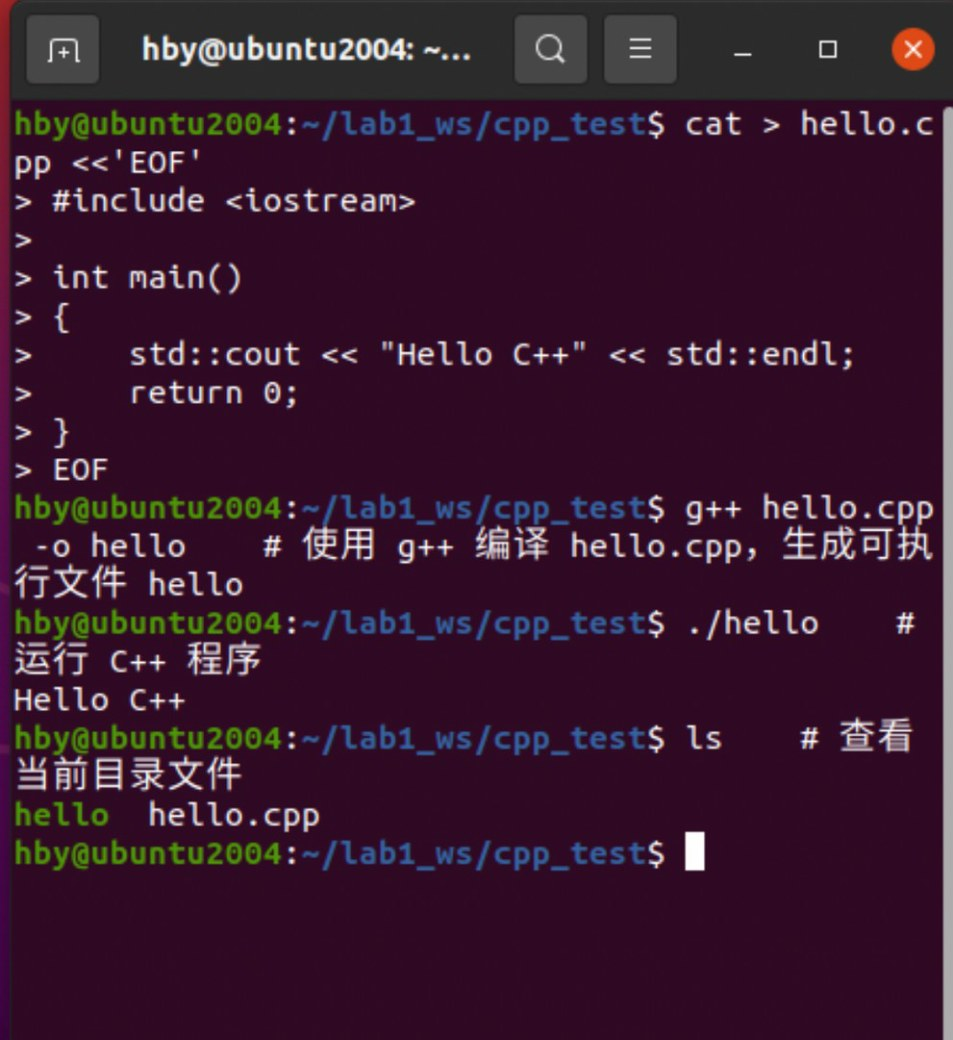
\includegraphics[width=0.42\textwidth]{figures/fig8_gpp.jpg}
\caption{使用 g++ 完成单文件 C++ 程序编译与运行}
\label{fig:gpp}
\end{figure}

\textbf{理解：}这一过程形成最小开发闭环：源文件 hello.cpp $\rightarrow$ g++ 编译 $\rightarrow$ 可执行文件 hello $\rightarrow$ ./hello 运行 $\rightarrow$ 检查输出。

\newpage

% ==================== 9 CMake 工程 ====================
\section{Part Three：CMake 工程构建测试}

\subsection{简单工程：cmake\_test}

在 cmake\_test 目录中编写 CMakeLists.txt 与 main.cpp，然后执行 cmake .、make、./hello。与直接使用 g++ 相比，CMake 更适合包含多个源文件的工程，可以统一描述构建规则。

\begin{lstlisting}[language=cmake]
cmake_minimum_required(VERSION 3.10)
project(cmake_test)
add_executable(hello main.cpp)
\end{lstlisting}

\begin{lstlisting}[language=bash]
cmake .
make
./hello
\end{lstlisting}

\begin{figure}[H]
\centering
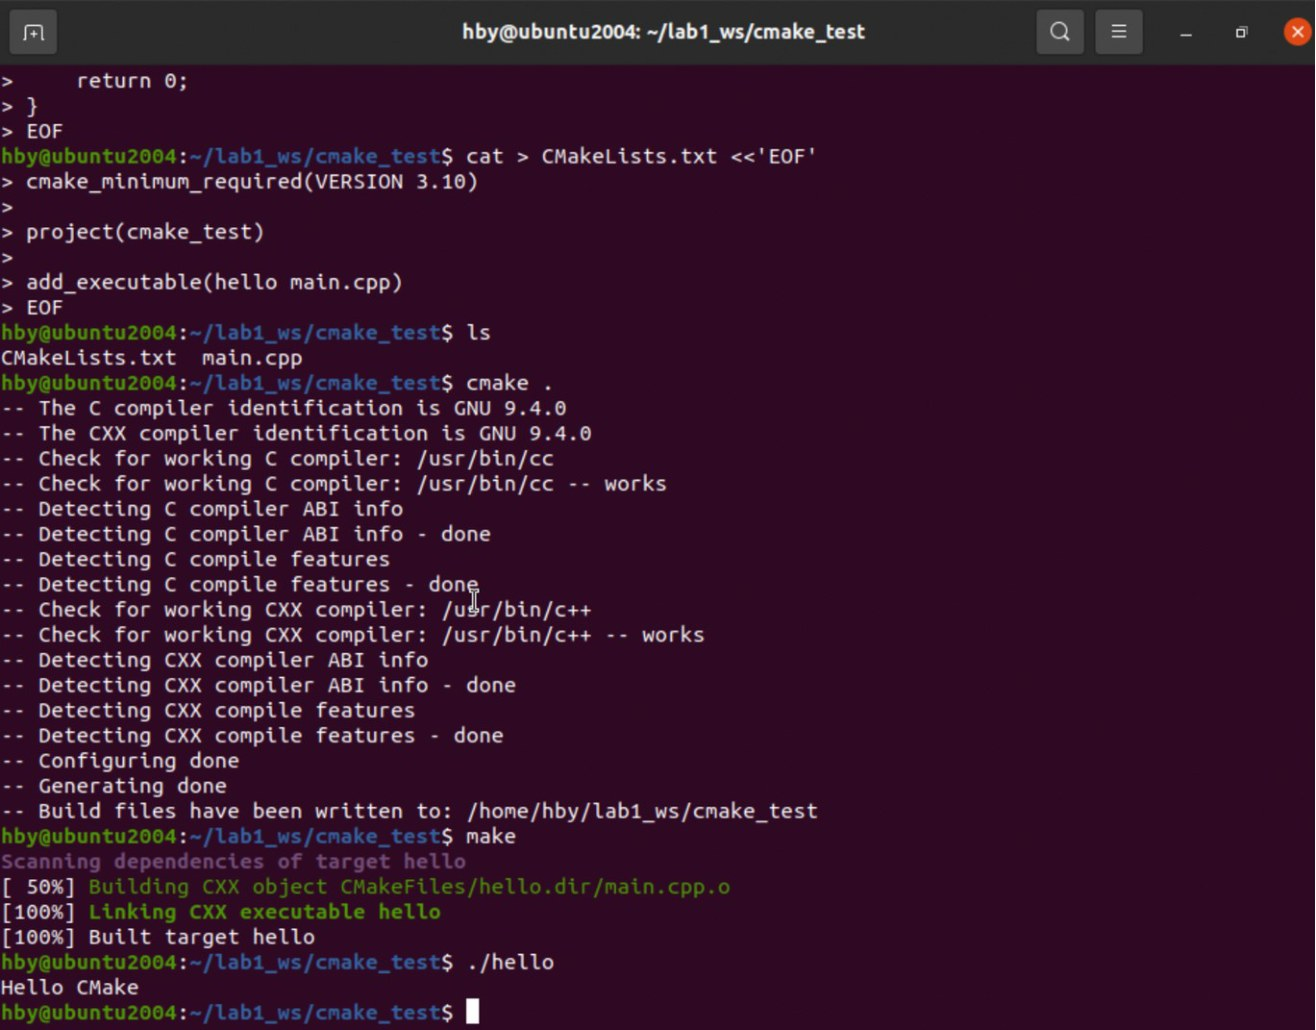
\includegraphics[width=0.56\textwidth]{figures/fig9_cmake.jpg}
\caption{使用 CMake 进行简单工程配置、构建与运行}
\label{fig:cmake_test}
\end{figure}

\subsection{多文件工程：lab1\_demo}

按老师示例建立 \textasciitilde/vnav-personal/lab1/lab1\_demo，包含 CMakeLists.txt、main.cpp、my\_lib.hpp、my\_lib.cpp。main.cpp 调用库函数，库函数返回 In library。文件名统一为 my\_lib，与 CMake 配置一致。

\begin{lstlisting}[language=cmake]
cmake_minimum_required(VERSION 3.10)
project(hello_world VERSION 1.0 LANGUAGES CXX)
add_library(mylib my_lib.cpp my_lib.hpp)
add_executable(main main.cpp)
target_link_libraries(main PRIVATE mylib)
\end{lstlisting}

\begin{lstlisting}[language=C++]
// main.cpp
#include <iostream>
#include "my_lib.hpp"
int main() {
    std::cout << "Hello world!" << std::endl;
    std::cout << my_lib_function() << std::endl;
    return 0;
}
\end{lstlisting}

\begin{lstlisting}[language=bash]
mkdir -p build
cd build
cmake .. && make && ./main
# Hello world!
# In library
\end{lstlisting}

\begin{figure}[H]
\centering
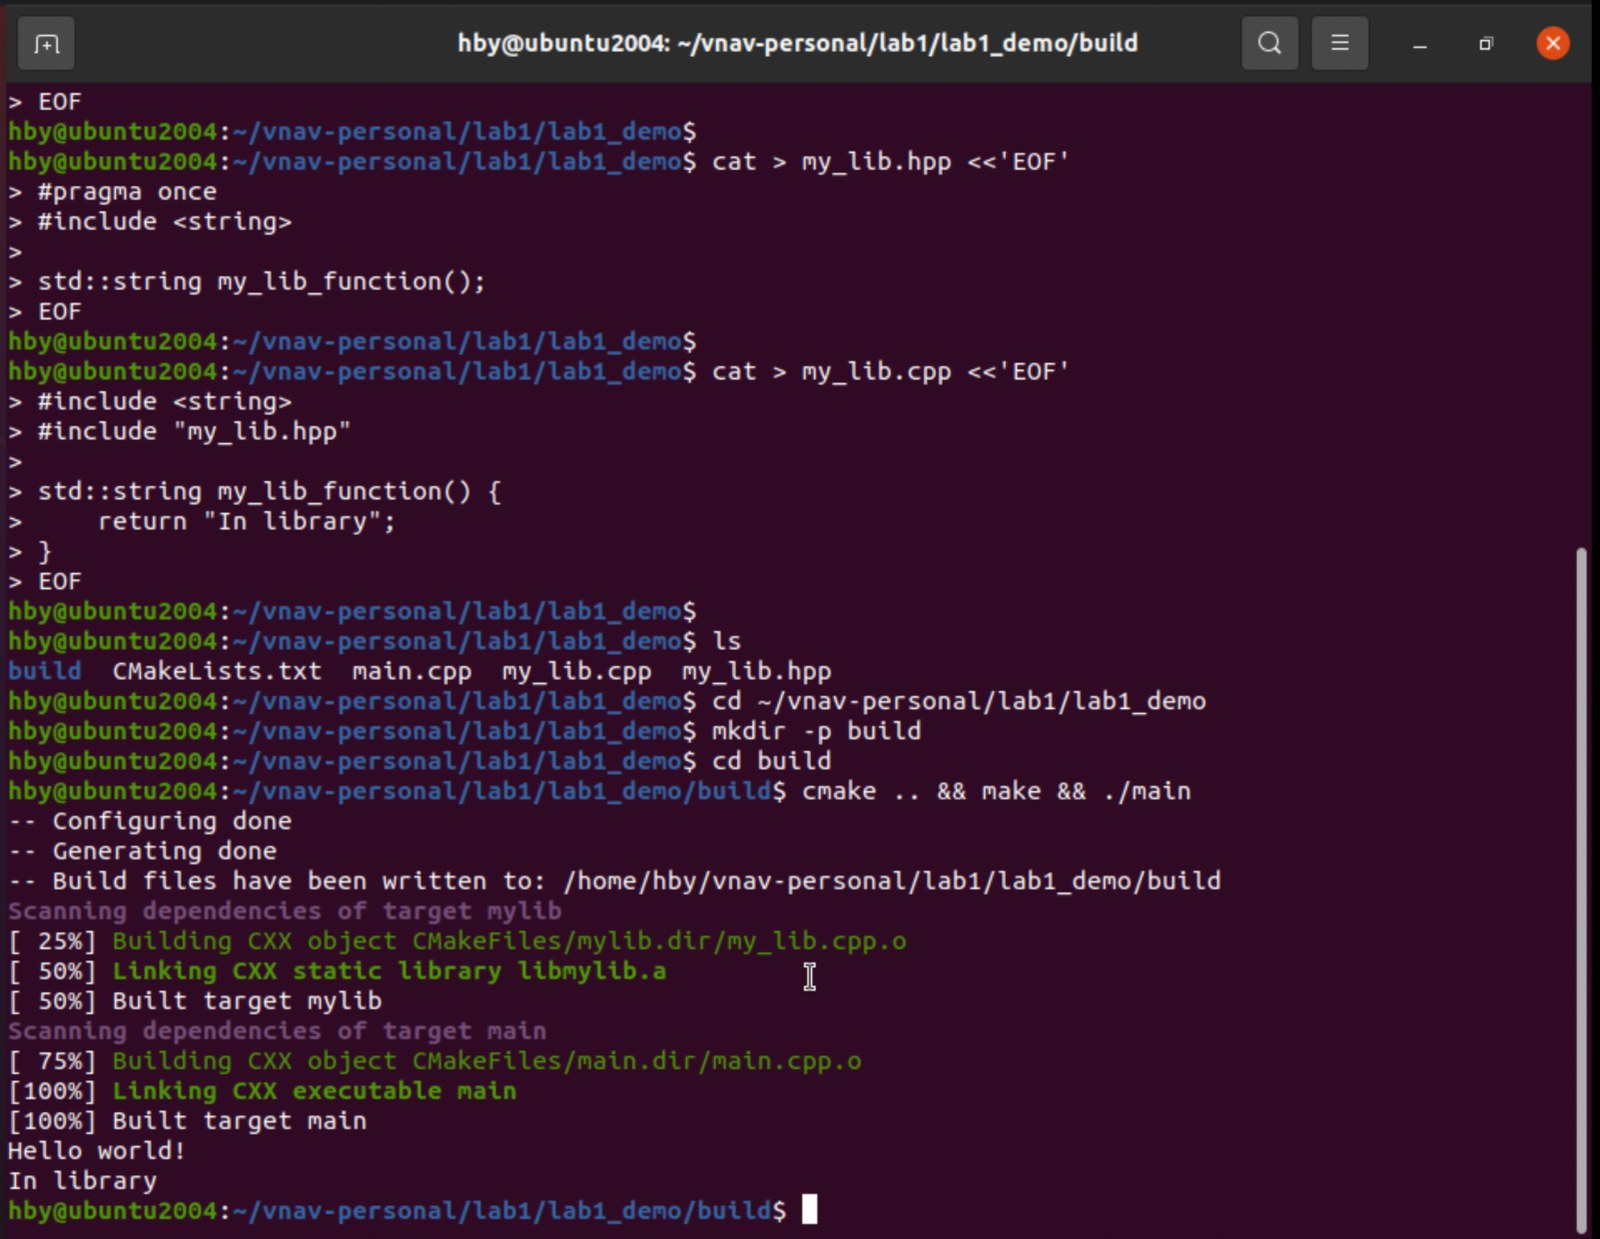
\includegraphics[width=0.58\textwidth]{figures/fig_lab1_demo.jpg}
\caption{多文件工程构建成功，输出 Hello world! 和 In library}
\label{fig:lab1_demo}
\end{figure}

\begin{center}
\begin{tabular}{p{2.6cm}p{11.2cm}}
\toprule
方式 & 适用场景与特点 \\
\midrule
g++ 直接编译 & 单文件/很小的程序，命令直接，适合快速测试 \\
CMake & 多文件/工程化项目，统一管理源文件、目标（库与可执行文件）和链接关系 \\
\bottomrule
\end{tabular}
\end{center}

\textbf{为什么机器人项目常用 CMake？}机器人项目通常包含多个源文件、库和依赖。CMake 能把构建规则集中管理，比逐条手写 g++ 命令更适合工程开发；add\_library 与 target\_link\_libraries 明确表达了库与可执行文件的链接关系。

\newpage

% ==================== 10 课程仓库与个人仓库 ====================
\section{Part Four：课程仓库与个人提交仓库}

\subsection{获取实验代码}

最初通过标准 HTTPS 地址克隆 MIT SPARK 提供的 VNAV-Labs 仓库（包含 lab1--lab9 全部实验）。最初曾使用不规范链接，系统要求输入 GitHub 用户名和密码；改用标准仓库地址后成功克隆。

\begin{lstlisting}[language=bash]
git clone https://github.com/MIT-SPARK/VNAV-labs.git
cd VNAV-labs && ls
cd lab1 && ls
\end{lstlisting}

\begin{figure}[H]
\centering
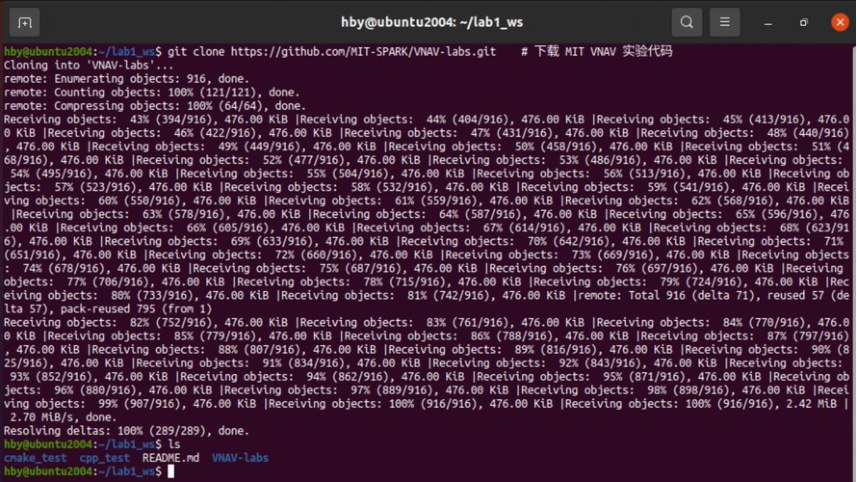
\includegraphics[width=0.52\textwidth]{figures/fig10_clone.jpg}
\caption{克隆 MIT VNAV-Labs 仓库成功}
\label{fig:clone_mit}
\end{figure}

随后按课程要求克隆课程仓库 ouc-vlab-course/vnav-codes 到 \textasciitilde/vnav-codes：
\begin{lstlisting}[language=bash]
git clone https://github.com/ouc-vlab-course/vnav-codes.git ~/vnav-codes
\end{lstlisting}

\begin{figure}[H]
\centering
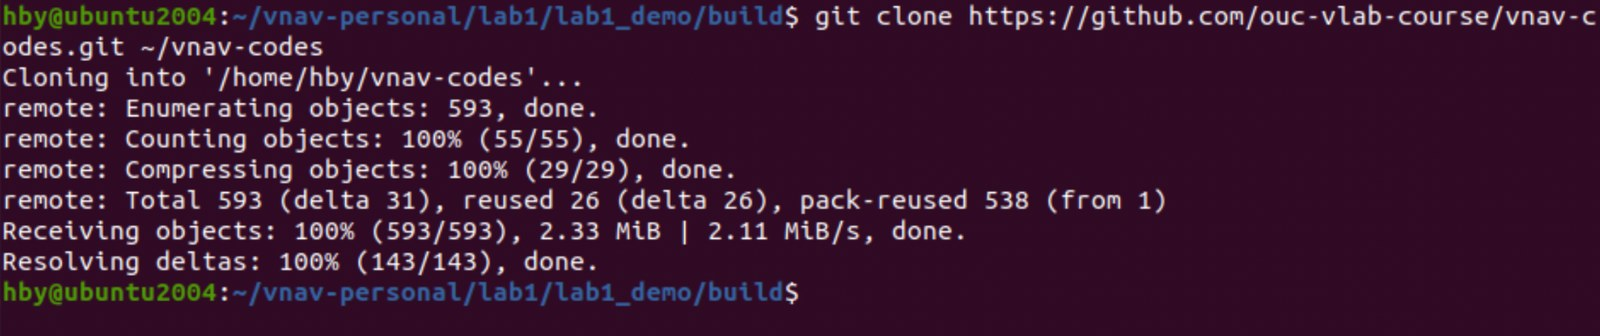
\includegraphics[width=0.88\textwidth]{figures/fig_clone_vnav_codes.jpg}
\caption{课程仓库克隆成功：593 个对象接收完成，143 个差异解析完成}
\label{fig:clone_course}
\end{figure}

\textbf{结果：}课程代码保存在 /home/hby/vnav-codes。课程仓库 lab1 目录包含 main.cpp、random\_vector.cpp、random\_vector.h 等文件，如图~\ref{fig:ls} 与图~\ref{fig:cat} 所示。

\begin{figure}[H]
\centering
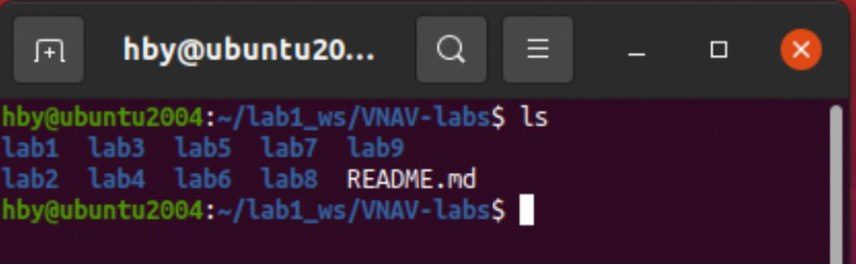
\includegraphics[width=0.44\textwidth]{figures/fig11_ls.jpg}\hfill
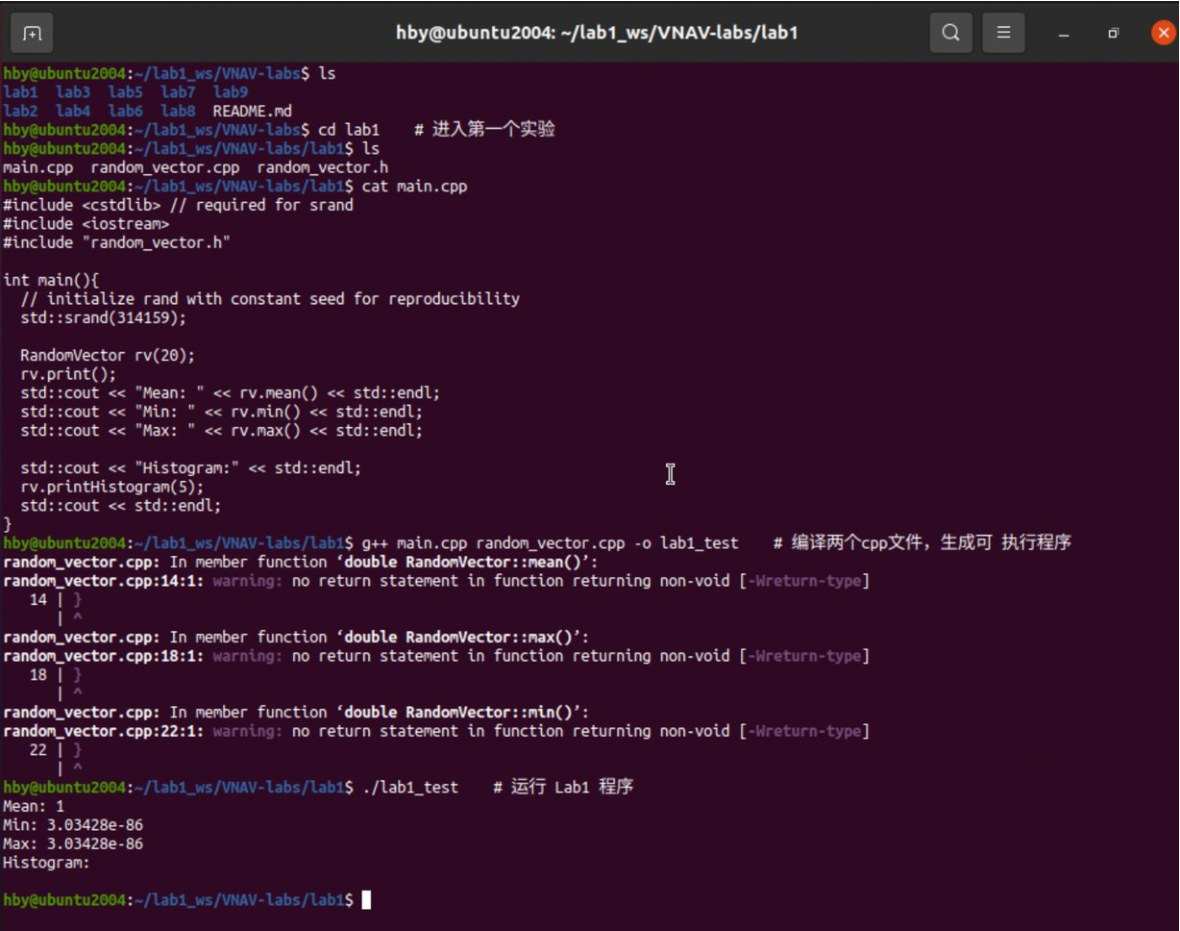
\includegraphics[width=0.44\textwidth]{figures/fig12_todo.jpg}
\caption{查看课程仓库目录结构与 lab1 源文件（main.cpp 中的 srand 与随机向量接口）}
\label{fig:ls}\label{fig:cat}
\end{figure}

\subsection{个人提交仓库 vnav-personal}

在 GitHub 上创建个人仓库 hbyhby123/vnav-personal，克隆到 \textasciitilde/vnav-personal，并在其中建立 lab1 目录，用于保存并推送全部练习成果（课程为校内课程，故使用 github.com 个人仓库替代 github.mit.edu 的组织仓库）。

\begin{lstlisting}[language=bash]
git clone https://github.com/hbyhby123/vnav-personal.git ~/vnav-personal
cd ~/vnav-personal && mkdir lab1
# 完成各练习文件后：
git add lab1 && git commit -m "..." && git push
\end{lstlisting}

个人仓库 master 分支已完成并成功推送的主要修订：
\begin{center}
\begin{tabular}{ll}
\toprule
提交 & 内容 \\
\midrule
bf9c003 & 完成 Lab1 全部练习文件 \\
da39796 & 添加 RandomVector 实现 \\
ad2d95a & 移除 algorithm 头文件，手写最大值/最小值循环 \\
3f7f490 & 新增 exercise1.txt，修正直方图分箱与输出方向 \\
55e790b & 新增 lab1\_demo 四个工程文件 \\
c6d80db & 追加五次 fortune 输出 \\
\bottomrule
\end{tabular}
\end{center}

最后检查 Git 状态时，仅 RandomVector 目录下的 random\_vector 可执行文件与 lab1\_demo 下的 build/ 目录为未跟踪项，均为编译产物；本次未将这些产物提交，仅提交源代码与练习答案文件。

\newpage

% ==================== 11 Shell 练习1 ====================
\section{Part Four：Shell 练习 1 --- dante.txt 文本统计}

\textbf{题目要求：}使用 wget 下载课程指定的 dante.txt（\url{https://raw.githubusercontent.com/dlang/dmd/master/druntime/benchmark/extra-files/dante.txt}），在 \textasciitilde/vnav-personal/lab1 创建 exercise1.txt，回答三个问题：共有多少行？共有多少个单词？有多少行不是空行？最后推送文件到 Git。

\begin{lstlisting}[language=bash]
wget https://raw.githubusercontent.com/dlang/dmd/master/druntime/benchmark/extra-files/dante.txt
wc dante.txt
grep -cv '^[[:space:]]*$' dante.txt
\end{lstlisting}

\begin{figure}[H]
\centering
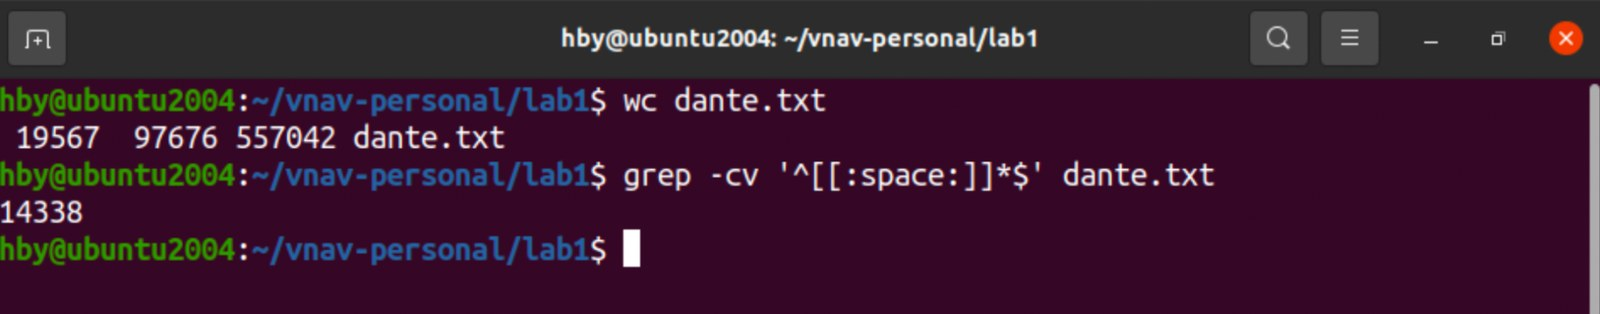
\includegraphics[width=0.92\textwidth]{figures/fig_dante_stats.jpg}
\caption{dante.txt 文本统计结果：19567 行、97676 词、14338 个非空行}
\label{fig:dante}
\end{figure}

统计结果：wc 默认输出 ``19567 97676 557042 dante.txt''，其中 19567 为行数，97676 为单词数，557042 为字节数。图中使用 grep -cv 统计非空行；之后又使用 grep 过滤并通过 wc -l 复核，结果同为 14338。

exercise1.txt 内容：
\begin{lstlisting}
Lines: 19567
Words: 97676
Non-blank lines: 14338
\end{lstlisting}

随后执行 git add exercise1.txt、git commit 与 git push，将结果推送到个人仓库（提交 3f7f490）。

\textbf{小结：}wc 的 -l 统计行数、-w 统计单词数；``非空行''需要先用 grep 过滤掉只含空白字符的行，再用 wc -l 计数，两者结合即可完整回答题目。

\newpage

% ==================== 12 Shell 练习2 ====================
\section{Part Four：Shell 练习 2 --- fortune 输出追加}

\textbf{题目要求：}使用 apt 安装 fortune-mod；安装后运行 fortune 查看一条谚语；再运行 fortune 5 次，每次把输出追加到 \textasciitilde/vnav-personal/lab1/fortunes.txt（不能覆盖重建文件）；最后推送文件到 Git。

\begin{lstlisting}[language=bash]
sudo apt install fortune-mod
fortune          # 查看一条谚语
fortune >> ~/vnav-personal/lab1/fortunes.txt   # 第 1 次追加
fortune >> ~/vnav-personal/lab1/fortunes.txt   # 第 2 次追加
fortune >> ~/vnav-personal/lab1/fortunes.txt   # 第 3 次追加
fortune >> ~/vnav-personal/lab1/fortunes.txt   # 第 4 次追加
fortune >> ~/vnav-personal/lab1/fortunes.txt   # 第 5 次追加
\end{lstlisting}

\begin{figure}[H]
\centering
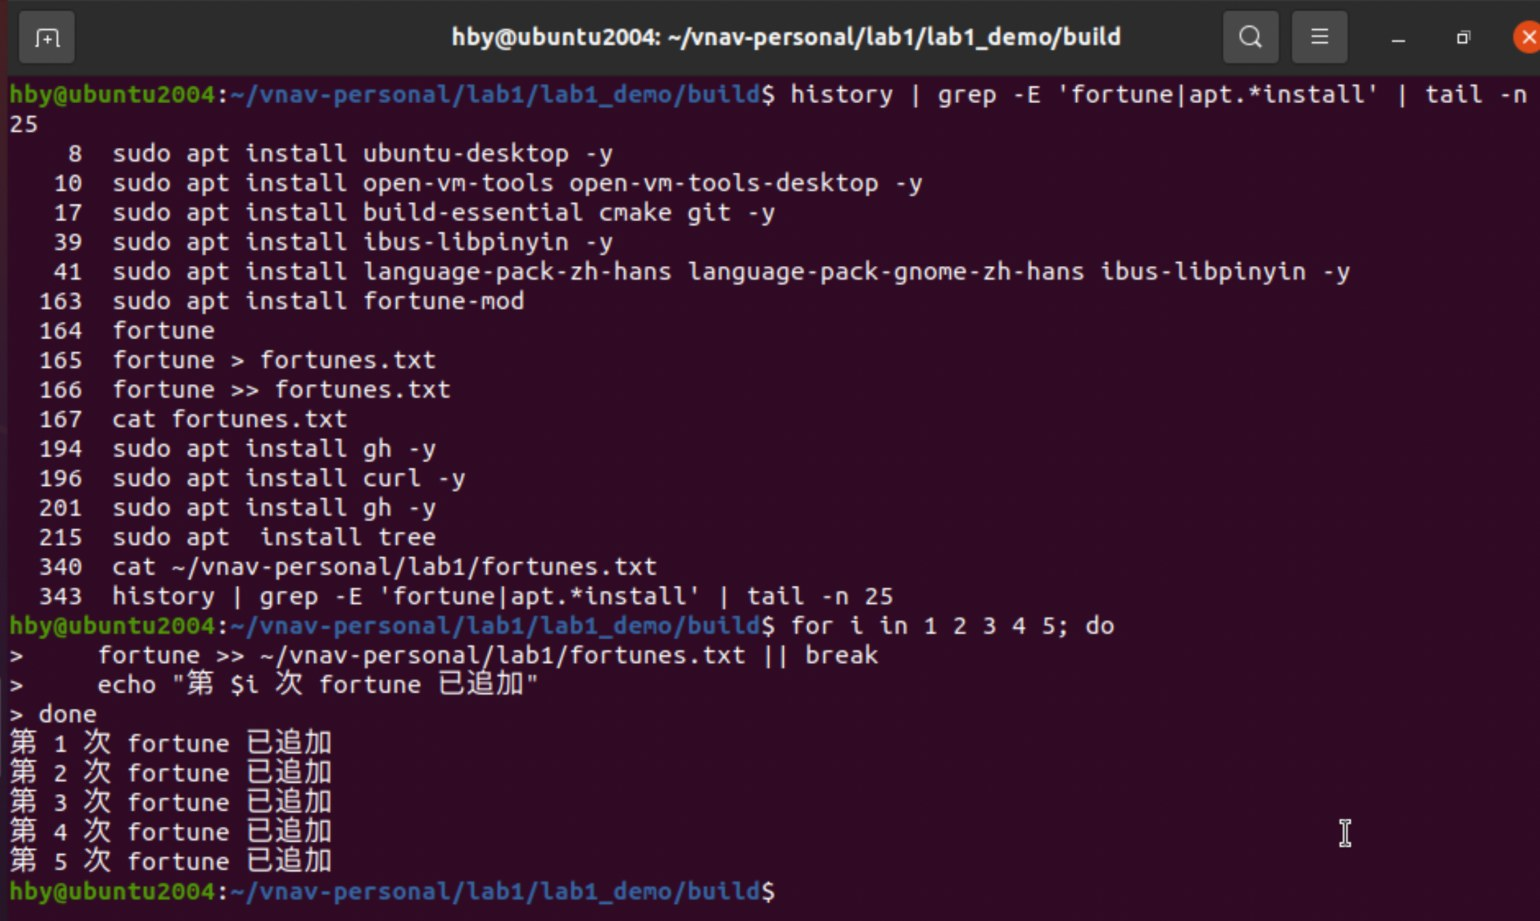
\includegraphics[width=0.56\textwidth]{figures/fig_fortune_history.jpg}
\caption{操作历史：fortune-mod 安装与 fortune 调用（五次追加均成功，已有内容保留）}
\label{fig:fortune}
\end{figure}

fortunes.txt 内容摘录（原有内容保留，新谚语追加在文件末尾）：
\begin{lstlisting}
You will have a long and unpleasant discussion with your supervisor.
Your sister swims out to meet troop ships.
A Tale of Two Cities LITE(tm)
	-- by Charles Dickens
...
Crime and Punishment LITE(tm)
	-- by Fyodor Dostoevski
...
Beware of a tall black man with one blond shoe.
April 1
	-- Mark Twain, "Pudd'nhead Wilson's Calendar"
...
\end{lstlisting}

随后执行 git add fortunes.txt、git commit 与 git push（提交 c6d80db）。

\textbf{小结：}``>'' 会覆盖文件内容，``>>'' 才会把输出追加到文件末尾。题目要求每次新增谚语都保留之前的输出，因此必须使用 ``>>''；成功提示在命令成功后输出，避免了把失败当成完成。

\newpage

% ==================== 13 C++ warmup ====================
\section{Part Four：C++ 热身题解答}

以下题目作答与 cpp-warmup.txt 一致，并补充了原答案中较简略的数值类型区别。

\subsection{Operators（运算符）}

\textbf{题 1：}下列代码运行后 i 和 j 的值分别是什么？
\begin{lstlisting}[language=C++]
int i = 0, j;
j = ++i;
j = i++;
\end{lstlisting}
\textbf{答：}初始 i = 0。j = ++i 先自增再赋值，i 变为 1、j 为 1；j = i++ 先赋值再自增，j 为 1、i 变为 2。\textbf{最终 i = 2，j = 1。}

\textbf{题 2：}下列代码打印什么？
\begin{lstlisting}[language=C++]
int i = 42;
std::string output = (i < 42) ? "a" : "b";
std::cout << output << std::endl;
\end{lstlisting}
\textbf{答：}i = 42，i < 42 为假，条件表达式选择冒号后的分支，打印 \textbf{b}。

\subsection{References and Pointers（引用与指针）}

\textbf{题 1：}
\begin{lstlisting}[language=C++]
int i;
int& ri = i;
i = 5;
ri = 10;
std::cout << i << " " << ri << std::endl;
\end{lstlisting}
\textbf{答：}ri 是 i 的引用，二者是同一个对象。ri = 10 之后 i 也为 10，打印 \textbf{10 10}。

\textbf{题 2：}
\begin{lstlisting}[language=C++]
int i = 42;
int* j = &i;
*j = *j**j;
std::cout << *j << std::endl;
\end{lstlisting}
\textbf{答：}*j**j 按从左到右解析为 (*j) * (*j)，即 42 × 42 = \textbf{1764}。*j 与 i 是同一个对象，因此 i 也变为 1764。

\textbf{题 3：}
\begin{lstlisting}[language=C++]
int i[4] = {42,24,42,24};
*(i+2) = *(i+1)-i[3];
std::cout << *(i+2) << std::endl;
\end{lstlisting}
\textbf{答：}*(i+2) 即 i[2]，*(i+1) 即 i[1]=24，i[3]=24，因此 i[2] = 24 - 24 = 0，打印 \textbf{0}。数组名 i 可隐式转换为指向首元素的指针，i[k] 等价于 *(i+k)。

\textbf{题 4：}
\begin{lstlisting}[language=C++]
void reset(int &i) {
    i = 0;
}
int j = 42;
reset(j);
std::cout << j << std::endl;
\end{lstlisting}
\textbf{答：}reset 的参数是引用，函数内 i = 0 直接修改实参 j，打印 \textbf{0}。引用参数避免了拷贝，也允许函数修改外部对象。

\subsection{Numbers（数值类型）}

\textbf{题 1：}int、long、long long 和 short 有什么区别？
\textbf{答：}它们都是整数类型，区别在于占用的存储空间和可表示的数值范围。C++ 标准只保证 sizeof(short) ≤ sizeof(int) ≤ sizeof(long) ≤ sizeof(long long)，最低位宽依次为 16、16、32、64 位，具体字节数由实现决定，因此不能把 long 永远写成固定 4 字节。常见 ARM64 Linux 上为 short 2、int 4、long 8、long long 8 字节。选择类型时应在满足数值范围的前提下尽量节省内存。

\textbf{题 2：}float 和 double 有什么区别？下面代码片段执行后 i 的值是多少？
\begin{lstlisting}[language=C++]
int i;
i = 3.14;
\end{lstlisting}
\textbf{答：}float 为单精度浮点（通常 32 位，约 6--7 位十进制有效数字），double 为双精度浮点（通常 64 位，约 15--16 位十进制有效数字），double 精度更高、范围更大。3.14 赋给 int 时向零截断小数部分，\textbf{i = 3}。

\textbf{题 3：}unsigned 和 signed 类型有什么区别？假设 char 为 8 位，下面代码片段中 c 的值是多少？
\begin{lstlisting}[language=C++]
unsigned char c = -1;
\end{lstlisting}
\textbf{答：}signed 类型可以表示负数、零和正数；unsigned 类型只表示非负整数，且溢出按模 2\textsuperscript{n} 回绕。8 位 unsigned char 的取值范围为 0--255，-1 转换为该类型相当于对 256 取模，\textbf{c = 255}。

\textbf{题 4：}下面代码片段运行后 i 的值是多少？
\begin{lstlisting}[language=C++]
int i = 42;
if (i) {
  i = 0;
} else {
  i = 43;
}
\end{lstlisting}
\textbf{答：}i = 42 非零，在条件中为真，执行 if 分支，\textbf{i = 0}。

\textbf{结果核对：}基础题结果已与 cpp-warmup.txt 对照，计算结果一致；本报告补充了原答案中较简略的数值类型区别。

\newpage

% ==================== 14 RandomVector 分析 ====================
\section{Part Four：RandomVector 类任务分析与实现}

\subsection{任务分析}

进入课程仓库 lab1 后，random\_vector.h 已给出类接口，random\_vector.cpp 中多个函数仍为 TODO。任务是根据接口和 main.cpp 的调用方式，补全 6 个成员函数。工程位于 lab1/RandomVector，main.cpp 固定使用随机种子 std::srand(314159)，因此每次运行得到相同的 20 个随机数，便于检查代码正确性。

\begin{lstlisting}[language=C++]
// random_vector.h（接口）
#include <iostream>
#include <vector>

class RandomVector{
  std::vector<double> vect;

  public:
    RandomVector(int size, double max_val = 1);
    void print();
    double mean();
    double max();
    double min();
    void printHistogram(int bins);
};
\end{lstlisting}

\begin{center}
\begin{tabular}{p{5.4cm}p{8.6cm}}
\toprule
函数 & 作用 \\
\midrule
RandomVector(int size, double max\_val=1) & 生成指定个数的随机数，并保存到 vect 向量中 \\
print() & 依次输出向量中的全部随机数 \\
mean() & 计算全部随机数的平均值 \\
max() & 寻找向量中的最大值 \\
min() & 寻找向量中的最小值 \\
printHistogram(int bins) & 按区间统计数据个数，并用 * 打印竖向直方图 \\
\bottomrule
\end{tabular}
\end{center}

\subsection{直方图的含义}

本实验在 min() 与 max() 之间划分 bins 个等宽区间，统计每个区间内有多少个随机数，再用星号 * 的数量表示该区间的数据个数，从最高层逐行向下输出竖向柱形。

\subsection{核心实现}

\begin{lstlisting}[language=C++]
RandomVector::RandomVector(int size, double max_val)
{
    for(int i = 0; i < size; i++)
    {
        double value = ((double)rand() / RAND_MAX) * max_val;
        vect.push_back(value);
    }
}

double RandomVector::mean()
{
    double sum = 0;
    for(double v : vect) sum += v;
    return sum / vect.size();
}

double RandomVector::max()
{
    double max_value = vect[0];
    for(double v : vect)
        if(v > max_value) max_value = v;
    return max_value;
}

double RandomVector::min()
{
    double min_value = vect[0];
    for(double v : vect)
        if(v < min_value) min_value = v;
    return min_value;
}
\end{lstlisting}

直方图统计核心逻辑：
\begin{lstlisting}[language=C++]
void RandomVector::printHistogram(int bins)
{
    if (bins <= 0 || vect.empty()) return;

    double low = min();
    double high = max();
    std::vector<int> histogram(bins, 0);

    for (double v : vect)
    {
        int index = 0;
        if (high > low)
        {
            index = static_cast<int>((v - low) / (high - low) * bins);
            if (index >= bins) index = bins - 1;
        }
        histogram[index]++;
    }

    int height = 0;
    for (int count : histogram)
        if (count > height) height = count;

    // 从最高层到最底层逐行输出：计数达到该层的区间打印 ***，否则打印空格
    for (int row = height; row > 0; row--)
    {
        for (int i = 0; i < bins; i++)
        {
            if (histogram[i] >= row) std::cout << "***";
            else std::cout << "   ";
            if (i < bins - 1) std::cout << " ";
        }
        std::cout << std::endl;
    }
}
\end{lstlisting}

\subsection{修正要点}

\begin{enumerate}[itemsep=1pt]
\item \textbf{删除 algorithm 头文件及其算法调用：}按课程要求不使用 <algorithm> 中的函数，最大值和最小值改用普通 for 循环逐个比较（提交 ad2d95a）。
\item \textbf{分箱范围由固定 0--1 改为当前向量的 min()--max()：}按题目要求``bins between min() and max()''等宽分箱（提交 3f7f490）。
\item \textbf{输出方向由横向改为竖向：}按老师示例逐行输出 *** 柱形，柱高等于最大计数值。
\item \textbf{边界处理：}bins ≤ 0 或空向量时直接返回；全部元素相等时（high == low）全部归入第一个箱；最大值归入最后一个箱，避免下标等于 bins。
\item \textbf{当前 mean/max/min 以非空向量为使用前提：}本次运行包含 20 个元素。
\end{enumerate}

\textbf{通俗理解：}RandomVector 可以理解为``一个保存随机数的类''：负责生成数据，并提供打印、平均值、最大/最小值和分布统计等功能。

\newpage

% ==================== 15 构建运行 ====================
\section{Part Four：RandomVector 编译、运行与结果分析}

补全 random\_vector.cpp 后，先使用 g++ 直接编译并运行，再使用 CMake 在 build 目录中完成构建并运行 lab1\_test。

\begin{lstlisting}[language=bash]
g++ -std=c++11 -Wall -pedantic -o random_vector main.cpp random_vector.cpp
./random_vector
\end{lstlisting}

\begin{lstlisting}[language=cmake]
cmake_minimum_required(VERSION 3.10)
project(vnav_lab1)
add_executable(lab1_test main.cpp random_vector.cpp)
\end{lstlisting}

\begin{lstlisting}[language=bash]
mkdir -p build && cd build
cmake .. && make && ./lab1_test
\end{lstlisting}

\begin{figure}[H]
\centering
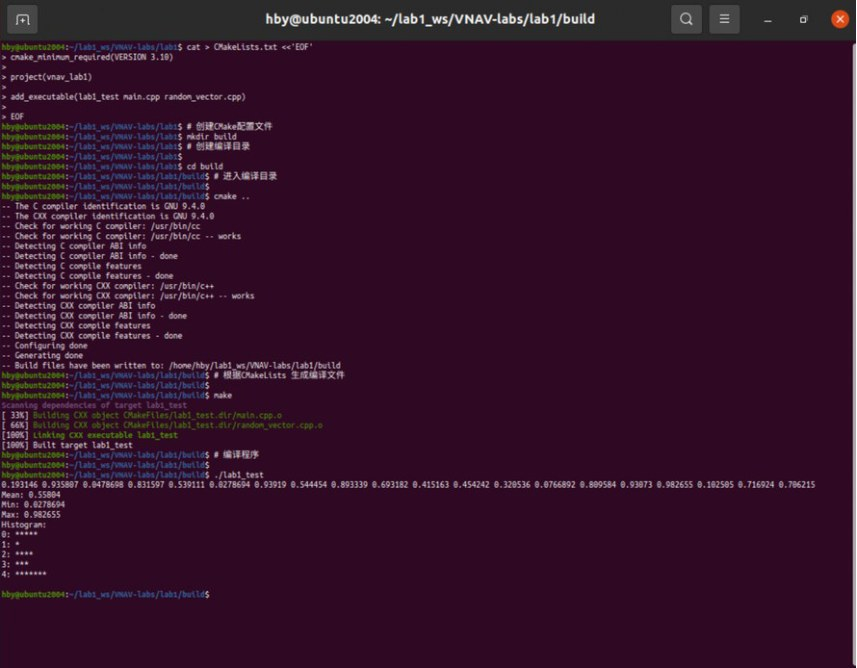
\includegraphics[width=0.54\textwidth]{figures/fig13_build_cmake.jpg}
\caption{在 build 目录中使用 CMake 构建并运行 Lab1}
\label{fig:build}
\end{figure}

最终运行结果（固定种子 std::srand(314159)，每次运行完全一致）：
\begin{lstlisting}
0.458724 0.779985 0.212415 0.0667949 0.622538 0.999018 0.489585 0.460587 0.0795612
0.185496 0.629162 0.328032 0.242169 0.139671 0.453804 0.083038 0.619352 0.454482
0.477426 0.0904966
Mean: 0.393617
Min: 0.0667949
Max: 0.999018
Histogram:
***     ***
***     ***
***     ***
***     ***
***     ***
***     ***
***     *** ***
*** *** *** *** ***
\end{lstlisting}

\begin{center}
\begin{tabular}{ll}
\toprule
指标 & 结果 \\
\midrule
随机数个数 & 20 \\
平均值 Mean & 0.393617 \\
最小值 Min & 0.0667949 \\
最大值 Max & 0.999018 \\
直方图区间数 & 5 \\
直方图统计（区间 0--4 的计数） & 8、1、8、2、1 \\
柱形最大高度 & 8 \\
\bottomrule
\end{tabular}
\end{center}

\textbf{可复现性：}本次运行固定使用 main.cpp 中的随机种子 std::srand(314159)，因此每次运行得到相同的 20 个随机数，便于检查代码正确性。该输出与课程网页给出的示例输出逐项一致（Mean: 0.393617、Min: 0.0667949、Max: 0.999018），说明实现与题目预期完全吻合。

\newpage

% ==================== 16 问题分析 ====================
\section{结果分布与问题分析}

\subsection{Histogram 结果}

本实验把当前向量的最小值 0.0667949 到最大值 0.999018 的范围等分为 5 个区间，统计每个区间内的随机数个数，如图~\ref{fig:hist} 与下表所示。

\begin{center}
\begin{tabular}{lll}
\toprule
区间编号 & 数值范围 & 数量 \\
\midrule
0 & [0.067, 0.253) & 8 \\
1 & [0.253, 0.440) & 1 \\
2 & [0.440, 0.626) & 8 \\
3 & [0.626, 0.813) & 2 \\
4 & [0.813, 0.999] & 1 \\
\bottomrule
\end{tabular}
\end{center}

\begin{figure}[H]
\centering
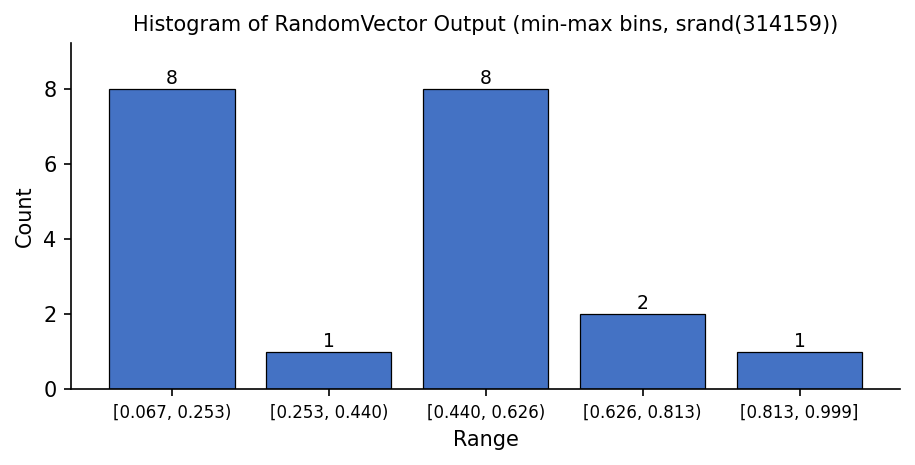
\includegraphics[width=0.68\textwidth]{figures/fig_hist_new.png}
\caption{根据最终输出整理得到的随机数据分布柱状图}
\label{fig:hist}
\end{figure}

20 个随机数在 0 到 1 之间分布较分散，其中 [0.067, 0.253) 与 [0.440, 0.626) 两个区间各有 8 个。由于样本数量只有 20 个，直方图不一定平滑，但足以验证 printHistogram() 的区间统计逻辑：五个区间计数之和 8+1+8+2+1 = 20，与向量长度一致。

\subsection{早期运行与最终版本的差异说明}

实验过程中的一次实际运行记录如图~\ref{fig:early} 所示：该次运行所用 main.cpp 尚未固定随机种子，输出为 Mean 0.55804、Min 0.0278694、Max 0.982655，五个柱子计数为 5、1、4、3、7，合计 20，与向量长度相符，编译输出未出现警告或错误。

\begin{figure}[H]
\centering
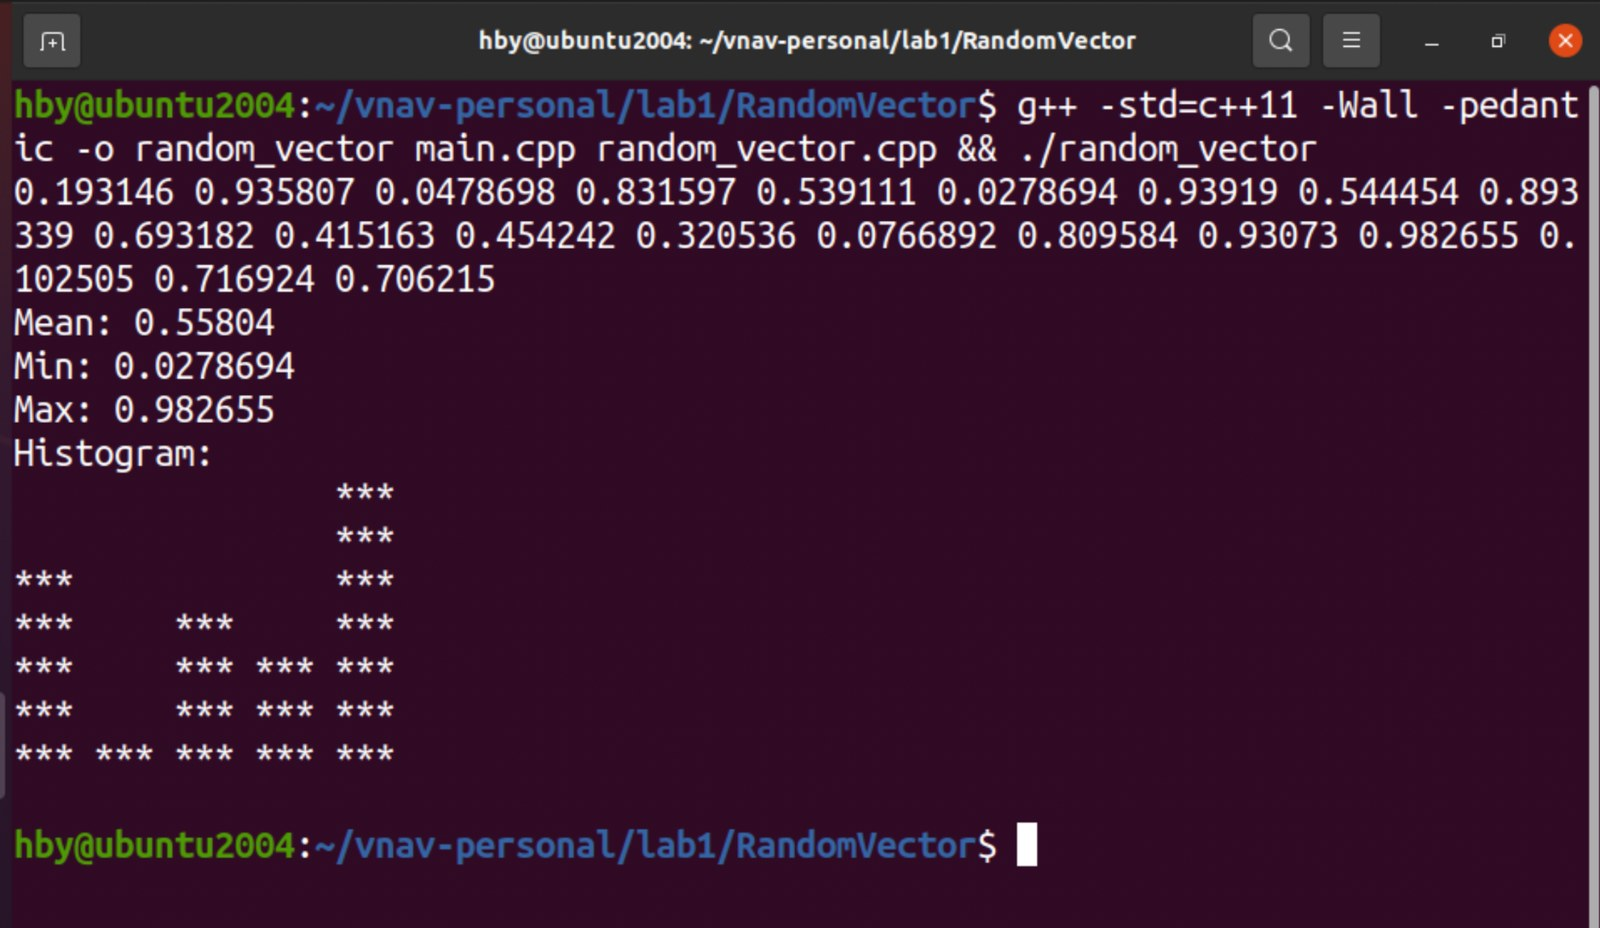
\includegraphics[width=0.70\textwidth]{figures/fig_early_run.jpg}
\caption{一次实际运行记录（未固定随机种子，输出与最终提交版不同）}
\label{fig:early}
\end{figure}

\textbf{说明：}随机数不同，平均值与直方图分布自然不同，这是正常现象。但若随机种子不固定，每次运行结果都不同，既不利于自查，也不便于老师复现批改。因此最终提交版本恢复使用课程原版 main.cpp 中的 std::srand(314159)，输出稳定为 Mean 0.393617（第 15 章），并与课程示例一致；直方图形状不必与老师示例完全一致，计数逻辑正确即可。

\subsection{实验中遇到的问题与解决方法}

\begin{center}
\begin{tabular}{p{4.6cm}p{4.2cm}p{6.2cm}}
\toprule
问题 & 原因 / 现象 & 解决方法 \\
\midrule
apt 更新出现 file:/cdrom 报错 & 软件源中残留光盘源条目 & 删除 /etc/apt/sources.list 中 cdrom 相关条目后重新 sudo apt update；本次进一步备份并切换清华源 \\
Mac 与 Ubuntu 输入法快捷键冲突 & Ctrl + Space 被 macOS 占用 & 调整输入法切换方式，实验中优先使用英文环境 \\
git clone 要求 GitHub 账号密码 & 最初使用了不规范地址 & 改用标准 HTTPS 仓库地址后正常克隆 \\
未实现 TODO 就编译 & 出现 no return statement 等警告并输出异常 & 按接口补全函数后重新编译运行 \\
首次启动只看到命令行 & 系统初次进入终端登录界面 & 正常登录、完成必要配置并重启后进入图形界面 \\
直方图方向与分箱不符合要求 & 早期实现横向输出、固定 0--1 分箱 & 改为竖向 *** 输出、min()--max() 等宽分箱（提交 3f7f490） \\
使用了 <algorithm> 头文件 & 课程要求不使用其中函数 & 删除 algorithm，手写循环求最大/最小值（提交 ad2d95a） \\
exercise1.txt 缺失 & 未创建 & 补充 wc 统计结果并提交（提交 3f7f490） \\
随机输出不可复现 & main.cpp 未固定随机种子 & 恢复课程原版 srand(314159)，输出稳定且与课程示例一致 \\
\bottomrule
\end{tabular}
\end{center}

\newpage

% ==================== 17 结论 ====================
\section{实验总结}

通过本次 Lab1 实验，我完成了以下工作：
\begin{enumerate}[itemsep=1pt]
\item 在 VMware Fusion 中安装 Ubuntu 20.04.5 ARM64 虚拟机，完成软件源备份并切换清华源；
\item 安装 build-essential、CMake、Git 并验证版本，掌握 Linux 常用命令（ls、cd、mkdir、echo、cat、wc、grep 等）；
\item 掌握 Git 基本版本管理（init、add、commit、log、clone、push），克隆课程仓库并建立个人提交仓库；
\item 掌握 g++ 单文件编译和 CMake 多文件工程构建方法（lab1\_demo 库与可执行文件链接）；
\item 完成 Shell 练习：dante.txt 统计（19567 行、97676 词、14338 个非空行）与五次 fortune 输出追加；
\item 完成 C++ 热身题（运算符、引用与指针、数值类型）并提交 cpp-warmup.txt；
\item 获取 MIT VNAV-Labs 与课程仓库代码，完成 RandomVector 类 6 个成员函数实现，删除 algorithm 依赖、按 min()--max() 等宽分箱、竖向输出直方图；
\item 最终程序在固定种子下稳定输出 20 个随机数、平均值、最大值、最小值以及直方图，与课程示例一致，实验目标全部完成。
\end{enumerate}

通过本次修订，解决了 exercise1.txt 缺失、直方图范围和方向不符合要求、多文件工程缺少实际运行证据等问题。理解了 ``>'' 覆盖与 ``>>'' 追加的差异，以及 CMake 中库与可执行文件的链接关系。后续应先核对当前目录再执行 Git 命令，并对照接口说明检查边界值，而不只检查程序能否运行。

\textbf{最终结论：}Lab1 已完成：Ubuntu 环境与清华换源、Linux 基础操作、Git 版本管理与仓库推送、C++ 编译、CMake 多文件构建、Shell 练习、C++ 热身题、RandomVector 实现及结果验证均已全部完成。

\end{document}
